\clearpage
\chapter{System testing}\label{ch:testing}
\begingroup
\clubpenalty=10000
\makeatletter\@clubpenalty=10000\makeatother
\widowpenalty=10000
\brokenpenalty=10000

The main comparisons depend on recovering anatomy from the right observations and measuring its change consistently. We therefore test the path from source masks and MRI inputs through model updates to the reported scores. Synthetic cases provide known answers, short real-data checks exercise the training path, and saved predictions allow independent scoring. Together, these checks support the distinction between recovering current anatomy and predicting future anatomy that runs through the report.

\section{Preserving geometry and physical volume}

Geometry tests cover axis flips, translations, anisotropic voxels and mismatched MRI-sequence grids. The loader checks finite image values and valid mask labels before measurement. Masks are aligned using their source and MRI transforms: resizing them independently as arrays can place otherwise valid labels in the wrong anatomical location.

Correct alignment alone does not preserve volume. Coarse nearest-neighbor sampling can discard a small labeled region even when the source mask contains positive volume. Across 322 inspected visits, coarse counting erased 605 of 7,728 regional compartment measurements. Among 5,784 regional changes, 102 reversed direction relative to source-volume aggregation. Figure~\ref{fig:6.1} shows these discrepancies across the fitting, selection and scoring partitions. A forecast trained on those targets could learn the effect of sampling rather than anatomical change.

\begin{figure}[!htbp]\centering
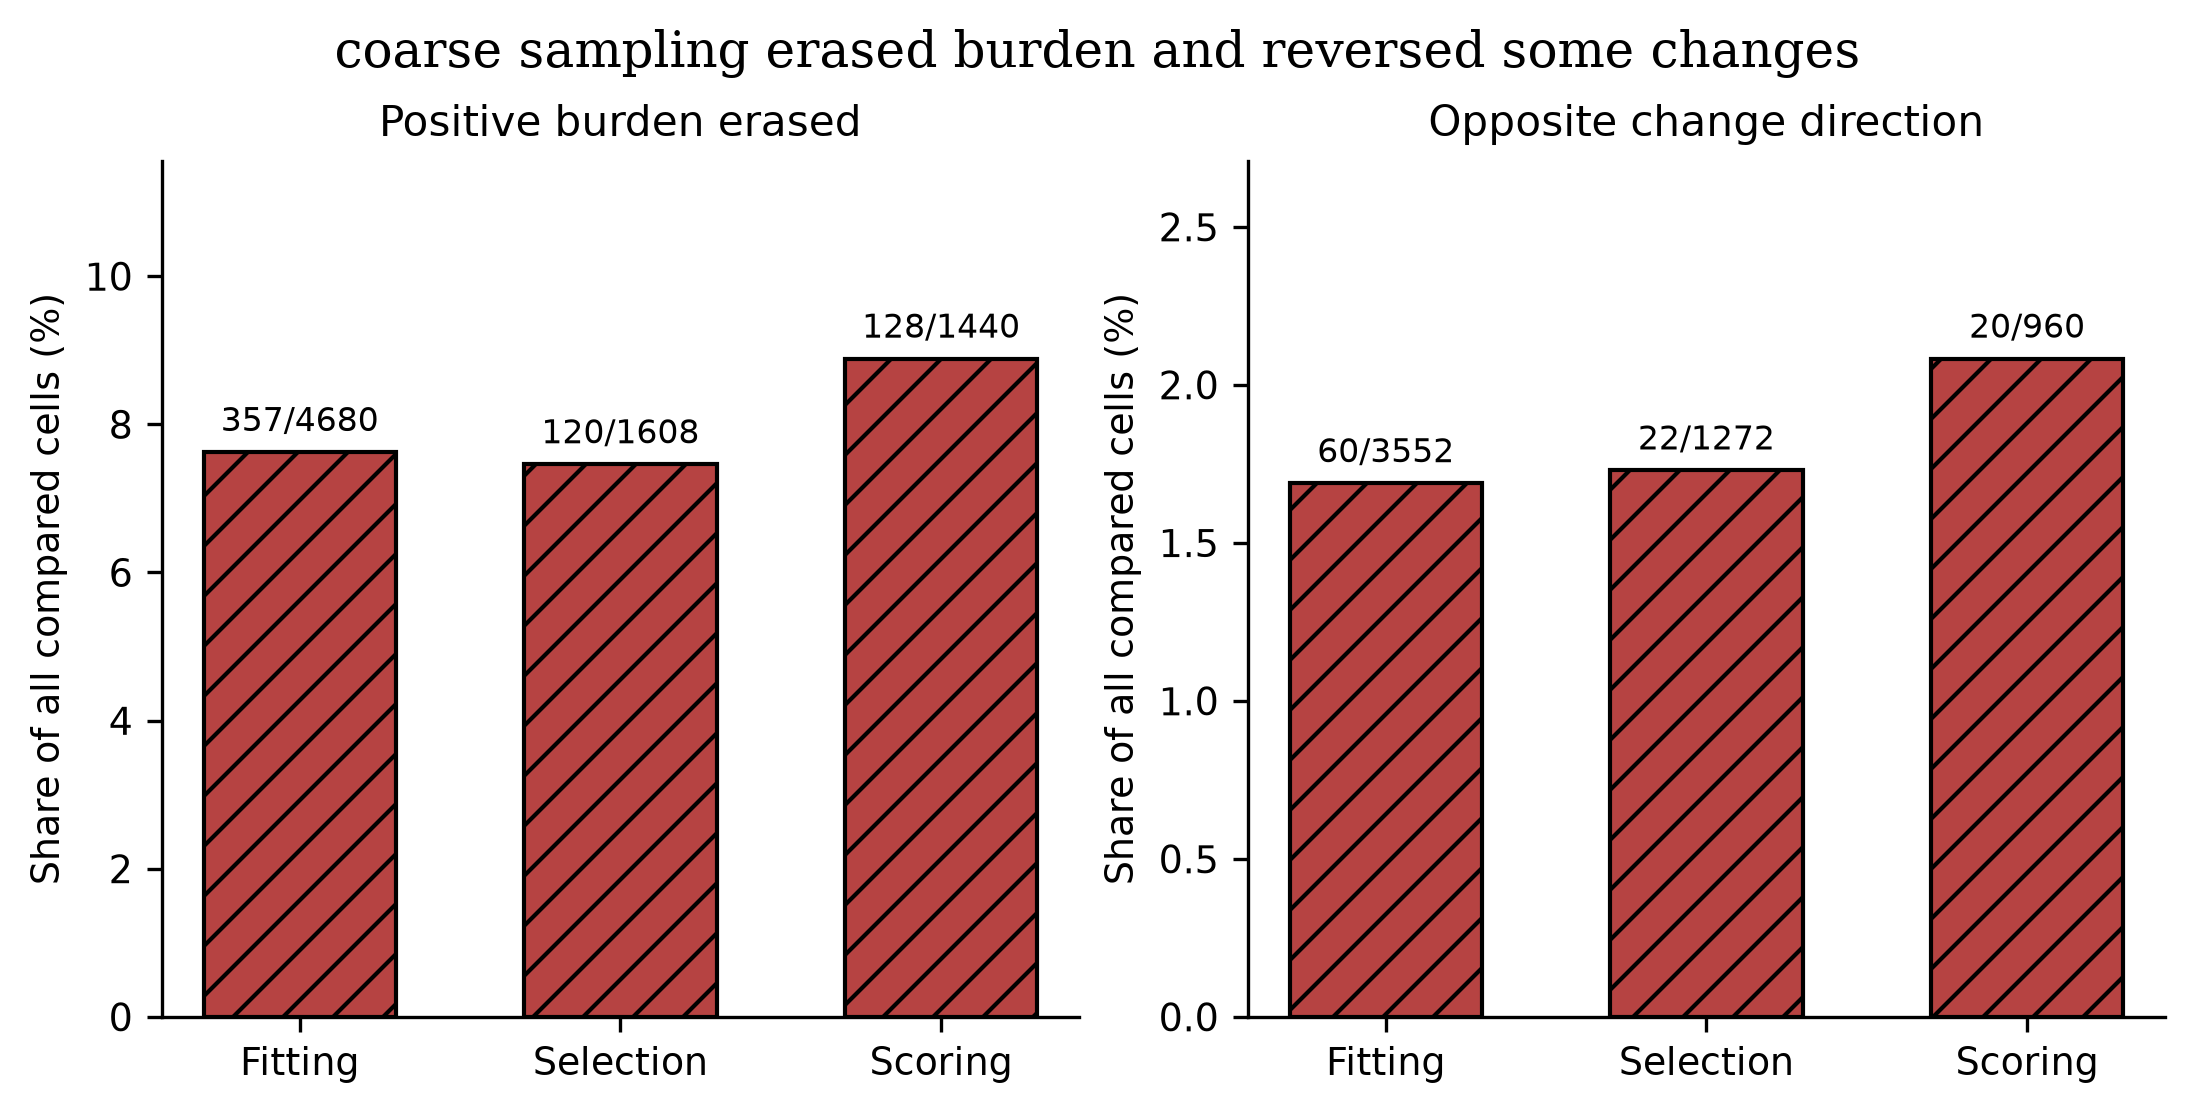
\includegraphics[width=\linewidth,height=0.57\textheight,keepaspectratio]{figures/figure_6_1.png}
\caption[Information lost through coarse mask sampling]{Regional target discrepancies across 322 visits. Each bar divides the number of affected region-compartment measurements or changes by all corresponding comparisons in that partition. Counts are printed beside the bars. These pooled counts describe the inspected cohort, with no sampling interval.}\label{fig:6.1}
\end{figure}

We measure regional volume by assigning each source voxel's physical volume to its region. Tests require regional and out-of-field totals to conserve the source total, preserve exact zeros for empty masks, and reject invalid labels. Independent extraction reproduced the regional volumes for all 322 visits. The targets retain physical units and visit order, and the regional regressions use newly fitted normalizers for these measurements.

\section{Enforcing the prediction cutoff}

Chronology checks preserve LUMIERE visit order using week bins and within-week suffixes. Forecast pairs refer to the original visit sequence, so removing an unusable intermediate scan cannot silently redefine the next visit. MU pairs require complete, increasing scan times.

A predictor must also be insensitive to information excluded by its cutoff. The tests replace future fields and verify that forecast inputs and predictions remain unchanged. Changing held-out outcomes must leave fitted parameters and predictions unchanged as well. These assertions address failure modes found during development: an earlier forecasting path admitted later-visit images, masks and interval features, and a clinical loader included eventual survival. The affected forecasting gains were withdrawn, and survival is excluded from default clinical inputs. Table~\ref{tab:6.1} summarizes the input and component checks.

\begingroup\singlespacing\small\setlength{\tabcolsep}{4pt}\renewcommand{\arraystretch}{1.25}
\begin{longtable}{>{\raggedright\arraybackslash}p{\dimexpr 0.5\linewidth-2\tabcolsep\relax}>{\raggedright\arraybackslash}p{\dimexpr 0.5\linewidth-2\tabcolsep\relax}}
\caption[Component and information-cutoff checks]{Assertions used to test model behavior and the information available at prediction time.}\label{tab:6.1}\\
\toprule \textbf{Test case} & \textbf{Expected behavior} \\\midrule\endfirsthead
\toprule \textbf{Test case} & \textbf{Expected behavior} \\\midrule\endhead
\bottomrule\endfoot
Padding and availability & Adding masked padding leaves the prediction unchanged; malformed availability flags are rejected. \\
Forward and backward pass & Outputs, losses and gradients remain finite; the intended trainable parameters receive gradients. \\
Frozen components & Frozen decoder or encoder parameters remain unchanged while gradients can reach the trainable predictor. \\
Checkpoint round trip & Saving and restoring the model reproduces its predictions and optimizer state. \\
Known metric fixture & CRPS agrees with a known analytic case; patient weighting matches an explicitly calculated result. \\
Future-input perturbation & Changing excluded future fields cannot alter the constructed forecast inputs or prediction. \\
Held-out-target perturbation & Changing held-out outcomes does not alter a fitted prediction or fitted model parameters. \\
\end{longtable}\endgroup

\section{Exercising training and saved states}

Short real-data checks exercise the complete training path: loading one or two batches, computing forward and backward passes, updating weights, and saving and restoring a checkpoint. They check finite losses and gradients, changes in trainable parameters, and preservation of frozen parameters. For FLAIR forecasting, replacing earlier images can change history predictions while leaving latest-only predictions fixed. Replacing withheld current FLAIR leaves the completion path unchanged. These checks establish that each comparison uses the intended inputs.

When a model improves little, fitting a few fixed examples helps distinguish a fitting problem from poor generalization. The FLAIR diagnostics use two patients for this purpose. A direct spatial-code diagnostic also bypasses the image encoder by optimizing its output codes. Chapter~\ref{ch:results} relates these fitting results to the completion and forecasting errors.

Acquisition tests follow the same principle at each sequence reveal. Unavailable images cannot enter the observed state, and changing reveal order must leave set fusion unchanged. Reloading a saved state reproduces its outputs; six inspected maps also reproduced their displayed native volumes. Hypothetical sequence features guide a choice, while actual revealed images determine the updated observation state.

\section{Scoring and reproducing predictions}

Comparable scores require the same target space and aggregation. Two latent comparisons mixed representation spaces, and their claimed 2.7-fold improvement was withdrawn after a same-space calculation. The representation-forecast ratios in Section~\ref{sec:initial-results} use patient-uniform errors for both the predictor and persistence, correcting an earlier mixture of pair-weighted ratios and patient-uniform absolute errors.

Metric tests use known numerical examples for CRPS and patient weighting. They also check empty targets and distinguish averaging seed scores from scoring an ensemble prediction. To reproduce a reported result, we restore parameters and normalizers, reconstruct predictions, and recalculate patient errors and paired intervals. Table~\ref{tab:6.2} gives the corresponding independent checks.

\begingroup\singlespacing\small\setlength{\tabcolsep}{4pt}\renewcommand{\arraystretch}{1.25}
\begin{longtable}{>{\raggedright\arraybackslash}p{\dimexpr 0.28\linewidth-2\tabcolsep\relax}>{\raggedright\arraybackslash}p{\dimexpr 0.72\linewidth-2\tabcolsep\relax}}
\caption[Prediction and measurement reproducibility]{Reconstruction of saved outputs and independent calculations of measurements and scores.}\label{tab:6.2}\\
\toprule \textbf{Comparison} & \textbf{Verification} \\\midrule\endfirsthead
\toprule \textbf{Comparison} & \textbf{Verification} \\\midrule\endhead
\bottomrule\endfoot
FLAIR completion and forecasting & Ninety complete prediction archives replayed exactly. Independent calculations reproduced the five primary contrasts and intervals, including tokens, normalizers, controls and scoring fields. \\
LUMIERE regional history & Thirty prediction arrays replayed exactly. Reconstruction covered 582 uses of measurements from 270 distinct visits. Three ridge solutions and selected penalties matched independent calculations. \\
MU measured history & Independent source-array counting reproduced volumes for 479 complete development visits. Nineteen prediction arrays, three selected ridge solutions and patient-bootstrap contrasts were checked. \\
Sequence addition & Nine selected checkpoints reproduced all 14,249 numerical assessment values. \\
Structured forecasting & Independent aggregation of 259 target records agreed within $1.5\times10^{-14}$. Anatomy and image outputs replayed exactly for four inspected forecast pairs. \\
\end{longtable}\endgroup

Resolution and intensity perturbations test sensitivity to the image input. Their interpretation depends on preprocessing: nonzero intensity standardization can largely cancel an affine intensity change. A fixed reduction in resolution tests the frozen-history predictor's dependence on image detail.

\section{Numerical stability and uncertainty}

The likelihood calculation must retain gradients for unlikely true labels. Taking a logarithm after flooring tissue probabilities gives zero gradient below the floor. Stable log-softmax and log-sum-exp calculations restore those gradients; the correction leaves saved-model inference outputs unchanged.

For equally weighted predictive samples, quantiles are computed from exact ranks. This avoids floating-point errors in cumulative weights selecting the wrong interval endpoint. The corrected calculation changes some conditional interval widths, while coverage and the quantity-model conclusions remain unchanged.

We also compare the saved 64-sample estimates with deterministic scores from the fitted quantity distributions. All 116 Gaussian family/target sample sets replayed exactly. This matters because a reproducible sample mean can still poorly approximate the mean of a heavy-tailed distribution. Chapter~\ref{ch:results} uses the exact distribution scores to assess that effect on forecast performance.

\endgroup
